% !Mode:: "TeX:UTF-8"

\begin{frame}{第二十二讲、曲线积分}
	\linespread{1.5}
	\begin{enumerate}
	  \item {\bf 内容与要求}{\b (\S 12.1)}
	  \begin{itemize}
		\item 理解曲线积分的概念
		\item 熟练掌握曲线积分的计算
		\item 掌握曲线积分的应用
	  \vspace{1em}
	  \end{itemize}
	  \item {\bf  课后作业:}
	  \begin{itemize}
	    \item {\b 习题12.1:10(1,3),12,13,15(2),23}
	  \end{itemize}
	\end{enumerate}
\end{frame}

\section{对弧长的曲线积分}

\begin{frame}{平面曲线的长度}
	\linespread{1.2}\pause
	\begin{exampleblock}{{\bf 例1:}求以下曲线的长度\hfill}
		\begin{enumerate}
		  \item $y=x^2,\;(0\leq x\leq 3)$
		  \item $\df{x^2}{a^2}+\df{y^2}{b^2}=1$
		\end{enumerate}
	\end{exampleblock}
	\pause
	{\bb 弧微分:}
	$$\d s=\sqrt{(\d x)^2+(\d y)^2}$$
	\pause
	{\bb 曲线长度:}
	$$s=\dint_L\d s$$
\end{frame}

\begin{frame}{空间曲线的长度}
	\linespread{1.2}
	设$L:\bm{r}(t)=(x(t),y(t),z(t)),\;(a\leq t\leq b)$,\pause 则
	$$\alert{\d s=\sqrt{(\d x)^2+(\d y)^2+(\d z)^2}\pause
	=\sqrt{(x'_t)^2+(y'_t)^2+(z'_t)^2}\d t} $$
	\pause 从而曲线长度
	$$\alert{s=\dint_L\d s\pause =\dint_a^b\sqrt{(x'_t)^2+(y'_t)^2+(z'_t)^2}\d t
	\pause =\dint_a^b|\bm{r}'(t)|\d t}$$
	\pause 
	\begin{exampleblock}{{\bf 例2}\hfill}
		计算圆柱螺旋线$x=\cos t,y=\sin t,z=t,(0\leq t\leq 2\pi)$的长度。
	\end{exampleblock}
\end{frame}

\begin{frame}%{对弧长的曲线积分及其应用}
	\linespread{1.2}
	\begin{exampleblock}{{\bf 例3}\hfill}
		已知空间曲线$L:\bm{r}(t)=(x(t),y(t),z(t)),\;(a\leq t\leq b)$,其上
		的线密度为$\mu(x,y,z)$,求:
		\begin{enumerate}
		  \item 曲线的质量
		  \item 曲线的质心
		  \item 关于$z$轴的转动惯量
		  \item 对位于$(a,b,c)$质量为$m$的质点的万有引力
		\end{enumerate}
	\end{exampleblock}
	\pause 
	{\bb 对弧长的曲线积分:}
	$$\alert{\dint_Lf(x,y,z)\d s=\dint_a^bf(x,y,z)|\bm{r}'(t)|\d t}$$
\end{frame}

\begin{frame}{对弧长的曲线积分的性质}
	\linespread{1.2}
	$$\alert{I=\dint_Lf(x,y,z)\d s=\pause\dint_a^bf(x,y,z)|\bm{r}'(t)|\d t}$$\pause
	{{\bf 约定:}计算对弧长的曲线积分时,应确保积分上限总是大于积分下限的。}\pause 
% 	\vspace{-1ex}
	\begin{enumerate}
	  \item {\bb 线性性}\pause 
	  \item {\bb 无向性:}\pause
	  $\dint_Lf(x,y,z)\d s=\dint_{L^-}f(x,y,z)\d s$\pause
% 	  \vspace{-1ex} 
	  \item {\bb 路径可加性}
% 	  \pause 
% 	  $$\dint_{L_1\cup L_2}f(x,y,z)ds=\left(\dint_{L_1}+\dint_{
% 	  L_2}\right)f(x,y,z)ds$$
	\end{enumerate}
% 	\alert{{\bf 注:}定积分可以视为对$x$轴的弧长的曲线积分}
\end{frame}

\begin{frame}{曲线积分的计算}
	\linespread{1.2}
	\begin{exampleblock}{{\bf 例4}\hfill}
		设有点$A(1,1,0)$和$B(1,1,1)$,$L$为线段$OA,AB$和$BO$组成的封闭曲线,
		方向为$O\to A\to B\to O$,计算曲线积分
		$$\oint_L(x+y+z)\d s.$$
	\end{exampleblock}
	\pause \alert{{\bf 计算步骤:}曲线(分段)参数化$\to$定限$\to$计算积分}
\end{frame}

\section{对坐标的曲线积分}

\begin{frame}{对坐标的曲线积分}
	\linespread{1.2}\pause
	\begin{exampleblock}{{\bf 例5}\hfill}
		已知某质点$M$在{\bb 引力场}
		$$\bm{F}(x,y,z)=(P(x,y,z),Q(x,y,z),R(x,y,z))$$
		中沿曲线$L:\bm{r}(t)=(x(t),y(t),z(t)),(a\leq t\leq b)$
		运动,求引力对其做的功。
	\end{exampleblock}\pause
	$$\alert{W=\dint_L\bm{F}\d\bm{s}=\dint_LP\d x+\dint_LQ\d y+\dint_LR\d z}$$
\end{frame}

\begin{frame}{对坐标的曲线积分}
	\linespread{1.2}
	$$\alert{W=\dint_L\bm{F}\d\bm{s}=\dint_LP\d x+\dint_LQ\d y+\dint_LR\d z}$$
	\pause{\bb 组合型曲线积分:}
	$$\alert{W=\dint_LP\d x+Q\d y+R\d z}$$
	\pause 其中,若$L$为封闭曲线,则可记为:
	$$W=\oint_LP\d x+Q\d y+R\d z$$
\end{frame}

\begin{frame}{对坐标的曲线积分的性质}
	\linespread{1.2}\pause
	\begin{enumerate}
	  \item {\bb 有向性:}\pause
	  $$\dint_LP\d x+Q\d y+R\d z=-\dint_{L^-}P\d x+Q\d y+R\d z$$
	  \pause
	  \item {\bb 路径可加性:}\pause 设$L=\bigcup_{k=1}^nL_k$,\pause 且$L$与$L_k(k=1,$
	  
	  $2,\ldots,n)$
	  方向均一致,\pause 则
	  $$\dint_LP\d x+Q\d y+R\d z=\sum\limits_{k=1}^n\dint_{L_k}P\d x+Q\d y+R\d z$$
	\end{enumerate}
\end{frame}

\section{曲线积分的计算}

\begin{frame}{曲线积分的计算}
	\linespread{1.2}
	\begin{exampleblock}{{\bf 例6}\hfill}
		设有点$A(1,1,0)$和$B(1,1,1)$,$L$为线段$OA,AB$和$BO$组成的封闭曲线,
		方向为$O\to A\to B\to O$,分别计算曲线积分
		$$\oint_L(x+y+z)\d s\quad\mbox{和}\quad\oint_Lx\d x+y\d y+z\d z.$$
	\end{exampleblock}
	\pause \alert{{\bf 计算步骤:}曲线(分段)参数化$\to$定限$\to$计算积分}
\end{frame}

\begin{frame}{两类曲线积分的关系}
	\linespread{1.2}
	设$L:\bm{r}(t)=(x(t),y(t),z(t)),\;(a\leq t\leq b)$,\pause 其单位切向量
	$$\bm{T}=\df{\bm{r}'(t)}{|\bm{r}'(t)|}$$
	\pause 则$\bm{T}$与$L$同向,\pause
	$$\alert{\dint_L\bm{F}\cdot \d\bm{s}=\dint_L\bm{F}\cdot\bm{T}\d s}$$
% 	=\dint_L\bm{F}\cdot\bm{r}'(t)\d t}$$
	\pause 即:\alert{对坐标的曲线积分总可以化为对弧长的曲线积分}
\end{frame}

\begin{frame}
	\linespread{1.2}
	\begin{exampleblock}{{\bf 例7}\hfill}
		计算曲线积分$\dint_Lxy\d x$,其中积分曲线$L$分别为:
		\begin{enumerate}
		  \item 由原点沿$y=x^3$至$A(1,1)$;
		  \item 由原点沿$y^2=x$至$A(1,1)$。
		\end{enumerate}
	\end{exampleblock}
\end{frame}

\begin{frame}
	\linespread{1.2}
	\begin{exampleblock}{{\bf 例8}\hfill}
		计算曲线积分$\dint_Ly\d x-x\d y$,其中积分曲线$L$分别为:
		\begin{enumerate}
		  \item 由$A(0,-1)$沿右半单位圆至$B(0,1)$;
		  \item 由$A(0,-1)$沿左半单位圆至$B(0,1)$;
		  \item 由$A(0,-1)$沿单位圆逆时针方向至$A(0,-1)$。
		\end{enumerate}
	\end{exampleblock}
\end{frame}

\section{曲线积分的应用}

\begin{frame}[<+->]{曲线积分的应用}
	\linespread{1.5}
	\begin{enumerate}
	  \item {\bf 对弧长的曲线积分:}
	  \begin{itemize}
	    \item 曲线的长度、质量
	    \item 曲线的质心、转动惯量
	    \item 曲线对质点的引力
	  \end{itemize}
	  \item {\bf 对坐标的曲线积分:}
	  \begin{itemize}
	    \item 变力沿曲线做功
	    \item \alert{向量场中的环量和流量}
	  \end{itemize}
	\end{enumerate}
\end{frame}

\begin{frame}{流量与环量}
	\linespread{1.2}
	考虑平面区域内$D$内的向量场
	$$\bm{v}=(P(x,y),Q(x,y)),\;(x,y)\in D.$$
	\pause $L:\bm{r}=\bm{r}(t)$为$D$内简单光滑闭曲线,\pause 取逆时针方向。\pause 
	
	$\bm{T},\bm{n}$分别为$L$的单位切向量和单位法向量。\pause 
	\begin{itemize}
	  \item {\bb 流量:}\pause $\ds\oint_L\bm{v}\cdot\bm{n}\d s$\pause
	  \alert{\;—“向量场穿过$L$的速率”}\pause 
	  \item {\bb 环量:}\pause $\ds\oint_L\bm{v}\cdot\bm{T}\d s$\pause
	  \alert{\;—“向量场环绕$L$的速率”}
	\end{itemize}
\end{frame}

\begin{frame}{几何解释}
	\linespread{1.2}
	\begin{columns}\pause 
		\column{.5\textwidth}
			\begin{center}
				\resizebox{!}{5cm}{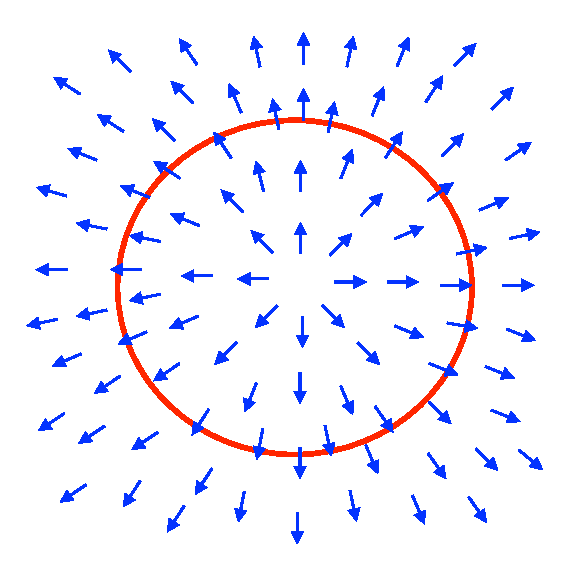
\includegraphics{./images/ch12/flow.pdf}}\pause 
				
				{\bb 流量:}$\alert{\ds\oint_L\bm{v}\cdot\bm{n}\d s}$\pause 
			\end{center}
		\column{.5\textwidth}
			\begin{center}
				\resizebox{!}{5cm}{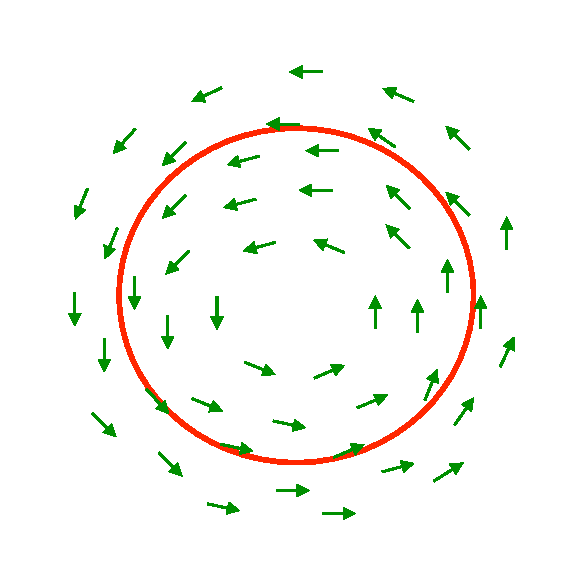
\includegraphics{./images/ch12/rotate.pdf}}\pause 
				
				{\bb 环量:}$\alert{\ds\oint_L\bm{v}\cdot\bm{T}\d s}$
			\end{center}
	\end{columns}
\end{frame}

\begin{frame}
	\linespread{1.2}
	\begin{exampleblock}{{\bf 例9}\hfill}
		分别计算向量场
		$$\bm{v}_1=(x,y)\quad\mbox{和}\quad \bm{v}_2=(-y,x)$$
		沿单位圆逆时针方向的流量和环量。
	\end{exampleblock}
\end{frame}

\begin{frame}[<+->]{小结}
	\linespread{1.4}
	\begin{enumerate}
	  \item {\bf 曲线积分的概念}
	  \begin{itemize}
	    \item 对弧长的曲线积分:无向性
	    \item 对坐标的曲线积分:有向性
	  \end{itemize}
	  \item {\bf 曲线积分的计算:}
	  \begin{itemize}
	    \item 曲线参数化$\to$定限$\to$积分
	  \end{itemize}
	  \item {\bf 曲线积分的应用}
	  \begin{itemize}
	    \item 曲线长度、质量
	    \item 转动惯量、质心、万有引力
	    \item 流量、环量
	  \end{itemize}
	\end{enumerate}
\end{frame}

%=====================================

% \begin{frame}{title}
% 	\linespread{1.2}
% 	\begin{exampleblock}{{\bf title}\hfill}
% 		123
% 	\end{exampleblock}
% \end{frame}
% 
% \begin{frame}{title}
% 	\linespread{1.2}
% 	\begin{block}{{\bf title}\hfill}
% 		123
% 	\end{block}
% \end{frame}